\chapter{Experiments}
\label{ExperimentsCh}

\section{Data}

\subsection{Dataset}

The dataset we have chosen to evaluate the models on is the Europarl dataset
between languages English and French. Europarl is a dataset of the proceedings
of the European Parliament, comprising in total of the 11 official languages of
the European Union.

The dataset was chosen as the number of sentences for English and French is
enough to be able to generalise (the uncompressed size of the full dataset is
619MB, 288MB for English, 311MB for French) to new sentences, and furthermore has
established baseline for NMT in the form of BLEU scores for all the different
language pairs in the full dataset, English-French in particular.\cite{koehn2005epc}

\begin{table}[t]
  \begin{center}
    \begin{tabular}{ |p{0.8\textwidth}| } 
      \hline
      \textbf{English}: I declare resumed the session of the European Parliament adjourned on Friday 17 December 1999, and I would like once again to wish you a happy new year in the hope that you enjoyed a pleasant festive period.\\
      \textbf{French}: Je déclare reprise la session du Parlement européen qui avait été interrompue le vendredi 17 décembre dernier et je vous renouvelle tous mes vux en espérant que vous avez passé de bonnes vacances.\\
      \hline
    \end{tabular}
    \caption{A randomly sampled sentence from the Europarl corpus}
  \end{center}
\end{table}

\subsection{Preprocessing}

The raw data is unfit for use directly with the model. For one thing the raw
data is in the form of strings and in order to use neural networks we need to
transform this into a form using vectors in some space $\mathbb{R}^m$.

From a linguistical point of view, a language contain a huge number of words at
any point in time. Furthermore, words never leave the language completely,
rather they go in and out of fashion and differ in how commonly they are use,
also depending on what context they are used in.

\begin{itemize}
\item We specify the maximum and minimum length of the words. This means that
  when training and testing, we can pad the shorter sentences with Null tokens
  until they are of the same length as the longest sentence.
\item We calculate the word frequencies in order to sort all of the words in the
  dataset in terms of how often it appear in absolute terms. This is then used
  to only retain the 30000 most common words. Words which are not part of this
  list gets replaced by an \texttt{<UNK>} token, specifying that it's an unknown
  word outside of the dictionary. This makes sure that only words which are
  prevalent enough such that the model can derive its relation to other words
  are part of the dictionary.
\item Newline characters were removed and replaced by \texttt{<EOS>},
  end-of-sentence tokens, signifying the end of a sentence.
\item In parts where we have a dataset of 2 or more language sentences in
  parallel, we make sure that both of the the languages both satisfy the above criteria.
\end{itemize}

It is important to note that due to how languages differ, even though the
dataset might consist of sentence pairs this will still not mean that in general
both of the languages will have the same dictionary of words. Partially this is
due to the different ways that languages are built up when expressing meaning,
but on a more basic level, there are no bijection between languages as words
have slightly different meaning and contexts, with some words only existing in
one language but not the other.

\section{Scores}

We will evaluate our models on a variety of scores:

\begin{description}
\item[ELBO] ELBO is the lower bound of the actual log-likelihood of the observed
  data
  \begin{equation*}
    \sum_{i=1}^{N} \log p_{\theta}(\bm{x}_i)
  \end{equation*}
\item[Qualitative] Since natural language is not a formal in the sense that it
  is ambiguous, inconsistent and with exceptions to rules; any of these scores
  will be imperfect insofar as taking into account the feel of the generated
  sentences. Due to this we will inspect the sentences manually.
\item[BLEU] BLEU compares the generated sentences with sentences translated by
  professional translators, yielding a score telling us how well the generated
  translation does in relation to the translated benchmarks for each sentence.

  We follow the thing as laid out in this link http://www.statmt.org/wpt05/mt-shared-task/\#TEST.
\item[KL] Part of our investigation is about building models that take into
  account the latent space, enforcing the model to encode the information in the
  latent variable z instead of the encoder/decoder part. Luckily, we have a
  quantitative measure of this, the KL divergence between the prior and the
  posterior q-distribution over $\bm{z}$,
  \begin{equation*}
    KL[q_{\phi}(\bm{z} | \bm{x}) || p_{\theta}(\bm{z})]
  \end{equation*}
  , where the KL is a measure of how much information is put into the
  q-distribution compared to just using the prior isotropic gaussian over
  $\bm{z}$, $p_{\theta}(\bm{z})$.
\item[Perplexity] After training the model we want the sentences in the test set
  to be probable under the probability distribution parametrised by
  $\bm{\theta}$. Perplexity is one measure of model fit. Given a sentence
  $\bm{w}_{1:L}$ the perplexity, $\text{PP}$, is defined as the per-word inverse
  probability,
  \begin{equation}
    \label{eq:perplexity}
    \text{PP}(\bm{w}_{1:L}) = p(\bm{w}_{1:L})^{-\frac{1}{L}}
  \end{equation}.
  In practice, this can be expressed in the form
  \begin{equation}
    \label{eq:perplexity_log_form}
    \text{PP}(\bm{w}_{1:L}) = \exp(-\frac{1}{L}\prod_{l=1}^L \log p(\bm{w}_l | \bm{w}_1, \dots, \bm{w}_{l-1}))
  \end{equation}
\end{description}

\section{Reconstruction}

We ran a couple of experiments on reconstruction as a proof of concept to show
that the model worked on data with only one language.

\begin{figure}[h]
  \centering
  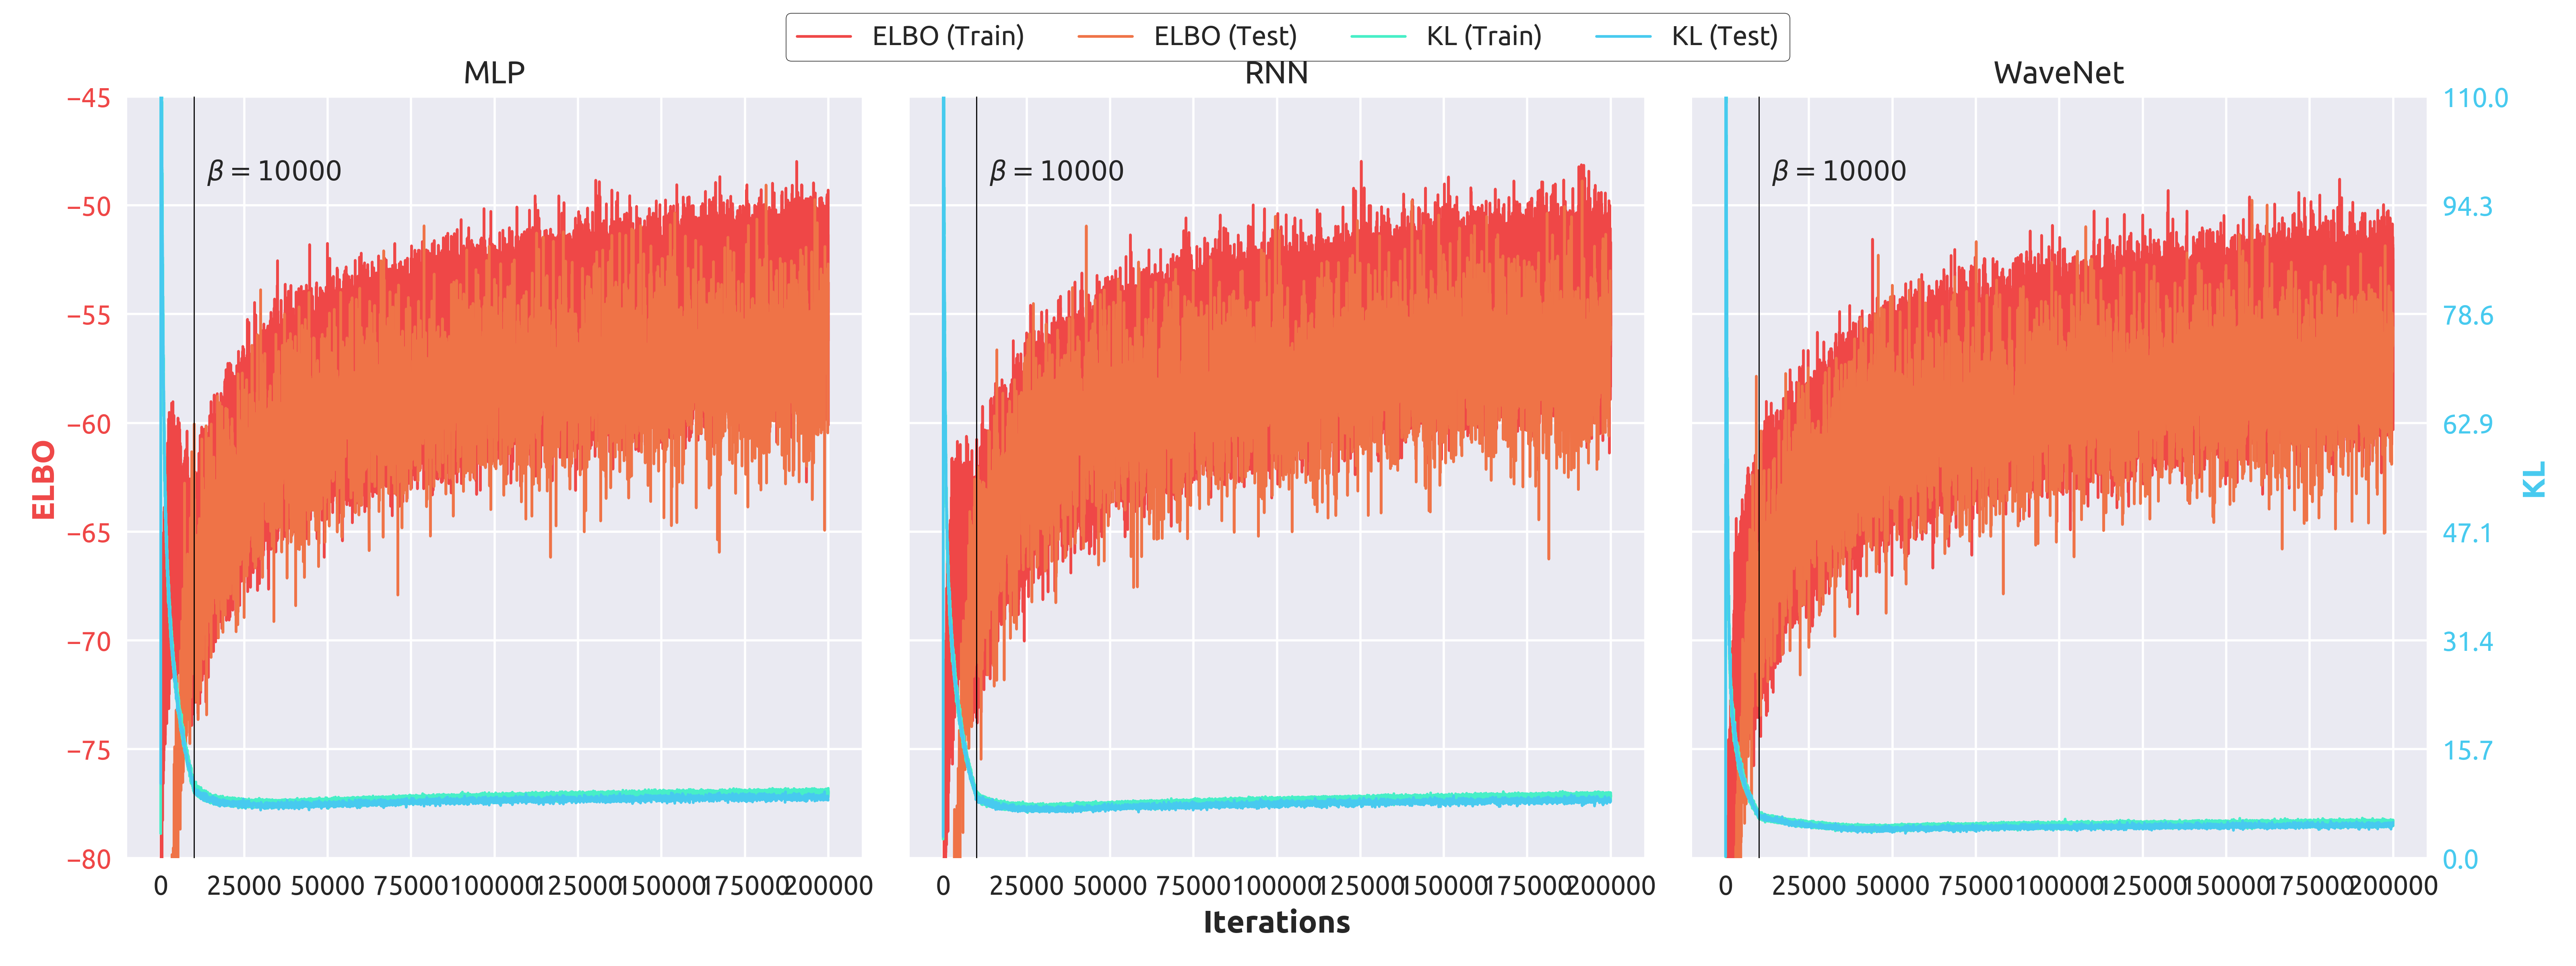
\includegraphics[width=\textwidth]{reconstruction_compare_fig.eps}
  \caption{Runs with various different recognition model}
  \label{fig:mlp_reconstruction_plot}
\end{figure}



\section{Translation}
